
%% ==================================================================================================
%%
\documentclass[12pt]{book}
\usepackage{amsfonts}
\usepackage{amsmath}
\usepackage{amssymb}
\usepackage{graphicx}
\usepackage{hyperref}
\usepackage{float}
\usepackage{verbatim}
\usepackage{xlop} %% for multiplication https://tex.stackexchange.com/questions/11702/how-to-present-a-vertical-multiplication-addition
\usepackage{listings} %% to format generic computer code
\usepackage{lmodern} % for bold teletype font
\usepackage{minted} % colour Java code

\usepackage{tasks}
%\NewTasks[style=enumerate,counter-format=tsk[A].,label-width=3ex]{choice}[\item](4)

%% =======   set page margins    =======
\setlength{\textheight}{10in}
\setlength{\textwidth}{7.4in}
\setlength{\topmargin}{-0.75in}
\setlength{\oddsidemargin}{-0.5in}
\setlength{\evensidemargin}{-0.5in}
\setlength{\parskip}{0.15in}
\setlength{\parindent}{0in}

%%  for European long division
% https://tex.stackexchange.com/questions/432435/how-to-set-up-european-french-style-long-division-in-tex
\newcommand\frdiv[5]{%
    \[
    \renewcommand\arraystretch{1.5}
    \begin{array}{l| l}
    #1 & #2 \\
    \cline{2-2}
    #3 & #4 \\
    \cline{1-1}
    #5 & \\
    \end{array}
    \]
}

%%  for European long division


%% ==================================================================================================

\begin{document}

%\title{ITI1100 Digital Systems I}
%\author{Kien Do 300163370}
%\date{Assignment \#1}
\newcommand{\reporttitle}{Laboratoire 3}
\newcommand{\reportauthorOne}{Kien Do}
\newcommand{\cidOne}{300163370}
\input{titlePage/titlepage.txt}



%% ==================================================================================================

%%%%%%%%%%%% PROBLEMS START HERE
\begin{enumerate}
    
    \item
    \begin{enumerate}
        \item Puisqu'une propriété d'un arbre est $n = 2e - 1$ où $n$ est le nombre de noeuds et $e$ est le nombre de noeuds externes, on a que $e = (n+1)/2$. Et puisqu'il y a 2567 noeuds, $e = (2567+1)/2 = 1284.$
        \item Puisqu'une propriété d'un arbre est $h \geq \log_{2}(n+1)-1$ où $h$ est la hauteur et $n$ est le nombre de noeuds, on a que $h \geq \log_{2}(2100+1)-1 \approx 10.03$. Par conséquent, $h=11$.
    
        \item Puisque $n \leq 2^{n+1}-1$ où $n$ est le nombre de noeuds,
        \begin{align*}
            n &\leq 2^{n+1}-1 \\
            n &\leq 2^{(11)+1}-1 \\
            n &\leq 2^{12}-1 \\
            n &\leq 4095
        \end{align*}
        Le nombre maximum de noeuds qu'il peut y avoir dans un arbre binaire complet de hauteur 11 est 4095.
    \end{enumerate}
    
    \item
    \begin{enumerate}
        \item
        \begin{enumerate}
            \item Pré-ordre: ABDHEJCGO
            \item Post-ordre: HDJEBOGCA
            \item In-ordre: HDBJEACGO
        \end{enumerate}
        \item 
        Voici le pseudocode:
        \begin{minted}[breaklines,frame=single]{java}
enqueue(root)
while (queue.size > 0):
    currNode = dequeue
    print(currNode.value)
    if (currNode.leftChild is not null)
        enqueue(currNode.leftChild)
    if (currNode.rightChild is not null)
        enqueue(currNode.rightChild)
        \end{minted}
        Voici mon travail brouillon\\\\
        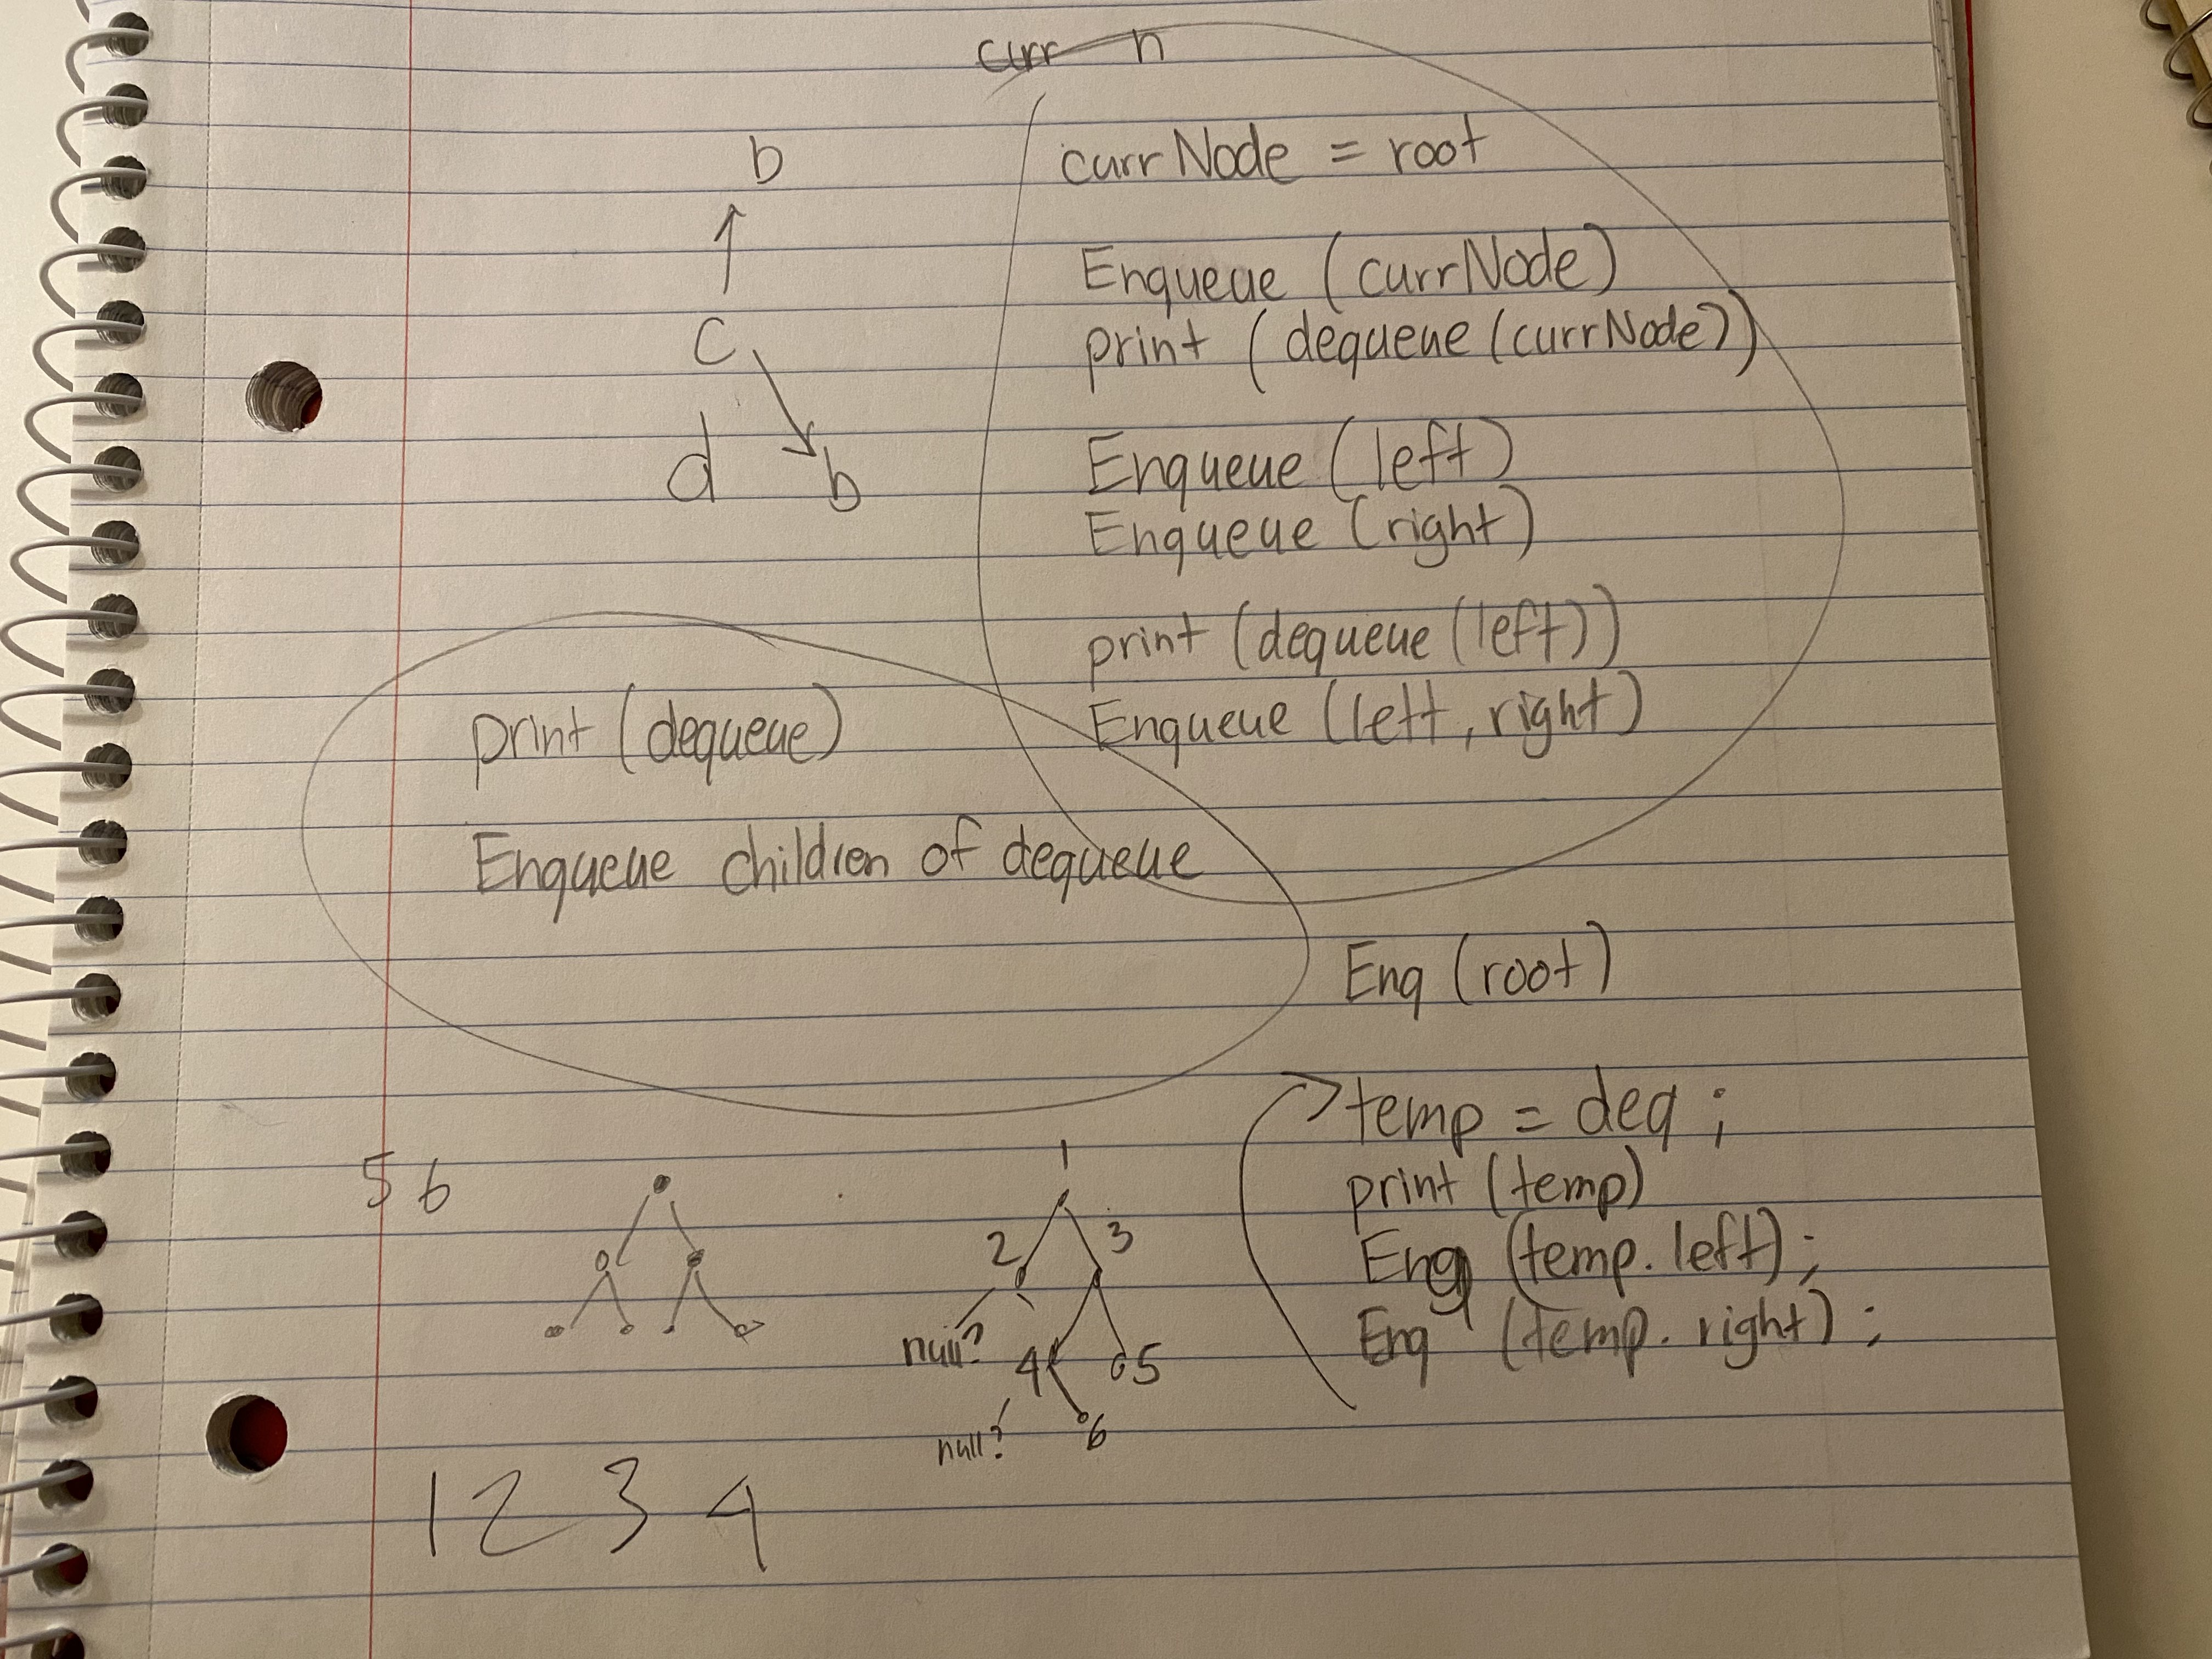
\includegraphics[scale=0.1]{csi2510lab3q2b.png}
        
        \item Inordre = [d c b e f a]\\Postordre = [d c f e b a]\\
        
        Puisque le parcours postordre met la racine à la fin, on peut déterminer que "$a$" est la racine. Maintenant qu'on sait la valeur de la racine, on peut déterminer les enfants gauches et droites de cet arbre en voyant la liste inordre. Toutes les enfants sur la gauche de $a$ dans la liste inordre viennent à la gauche, et toutes les enfants sur la droites viennent à la droite. Par conséquent, les noeuds enfants gauches sont [d c b e f] et il n'y a pas de noeuds enfants sur la droite parce que le noeud $a$ est déjà le noeud le plus 1a droite dans la liste.\\
        
        \includegraphics[scale=0.07]{csi2510lab3q2c0.png}\\
        
        Maintenant, on revoit la liste postordre et on trouve le prochain noeud. Dans ce cas, c'est le noeud $b$. Donc, on sait l'enfant gauche de $a$ est $b$. Mais quel sonts les enfants gauches et droites de $b$? Il faut voir les noeuds restant (les noeuds qui ne sont pas encore mis sur l'arbre) dans la liste inordre - les noeuds qui sont à la gauches de $b$ viennent à la gauche, et les noeuds qui sont à la droites de $b$ viennent à la droites. Donc, en voyant la liste inordre, les enfants gauches de $b$ sont [d c] et les enfants droites de $b$ sont [e f] (comme déjà mentionné, $a$ n'est pas inclus car $a$ est déjà mis sur l'arbre).\\
        
        \includegraphics[scale=0.07]{csi2510lab3q2c0.png}\\
        \newpage
        Si on continue ces étapes, on aura quelque chose comme cela ci-dessous,\\
        
        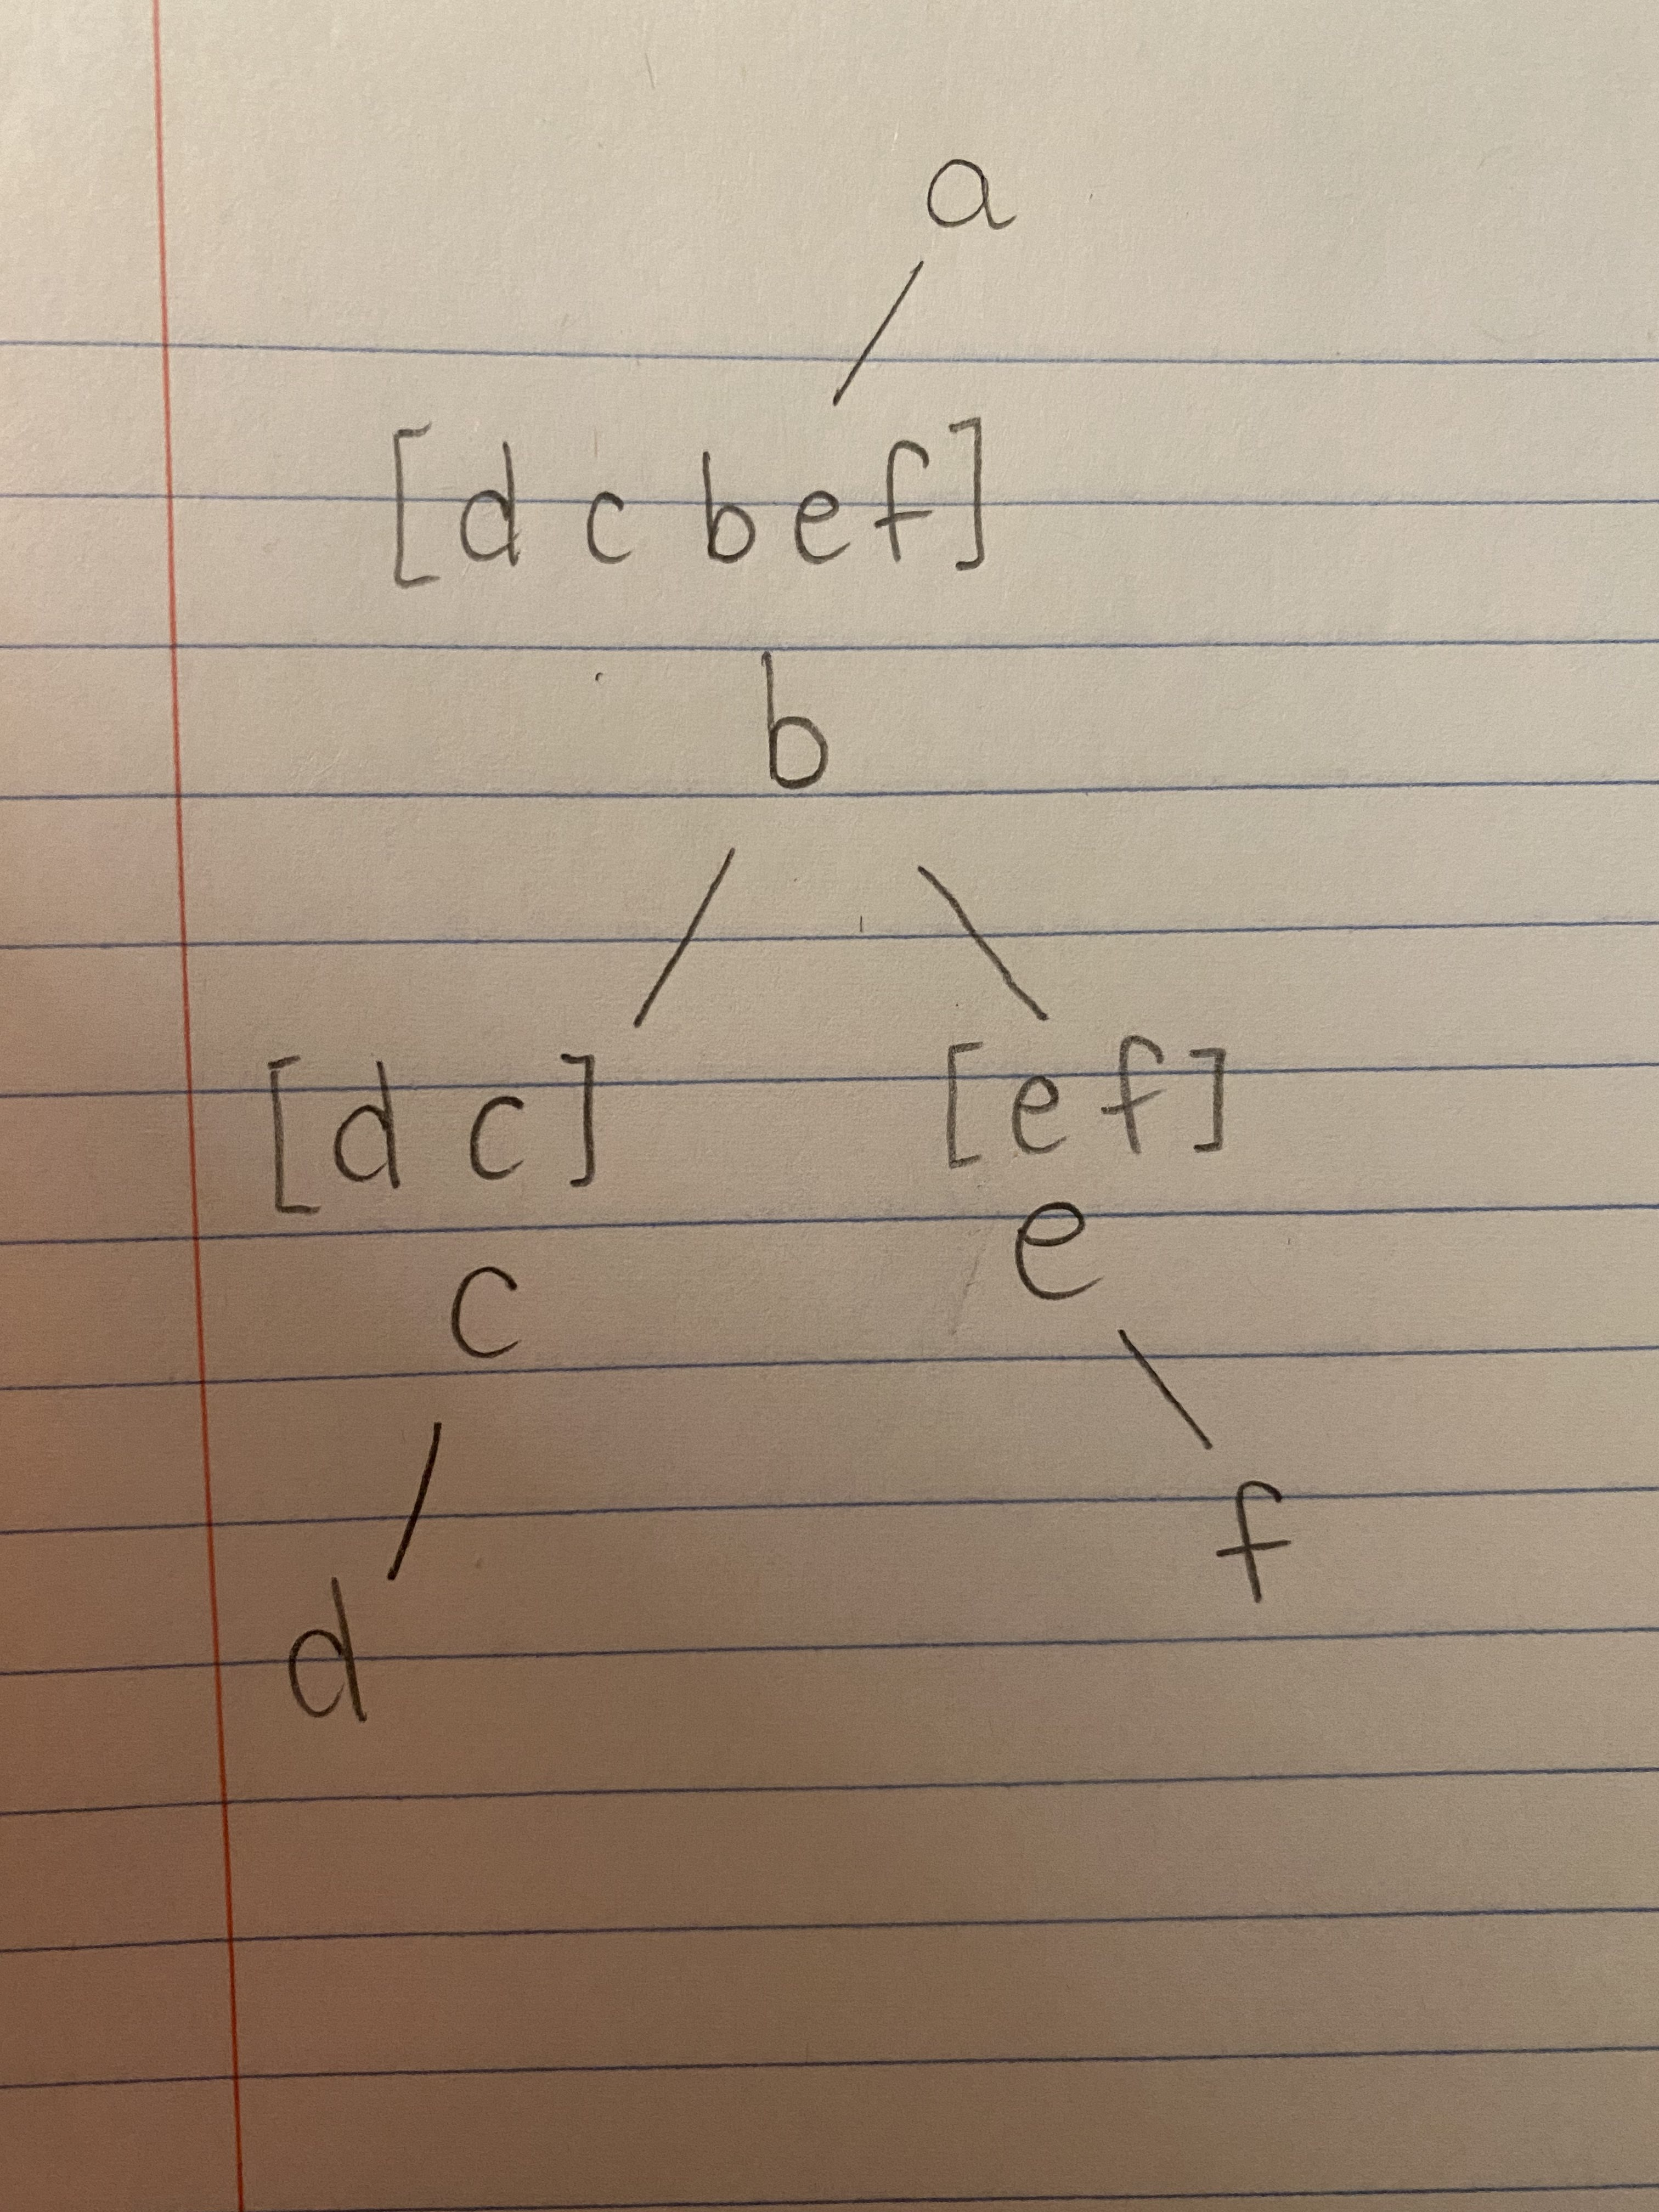
\includegraphics[scale=0.05]{csi2510lab3q2c2.png}\\
        
        Finalement, on termine avec un arbre comme cela. Les listes de parcours inordre et postordre fonctionnent avec cet arbre.
        
        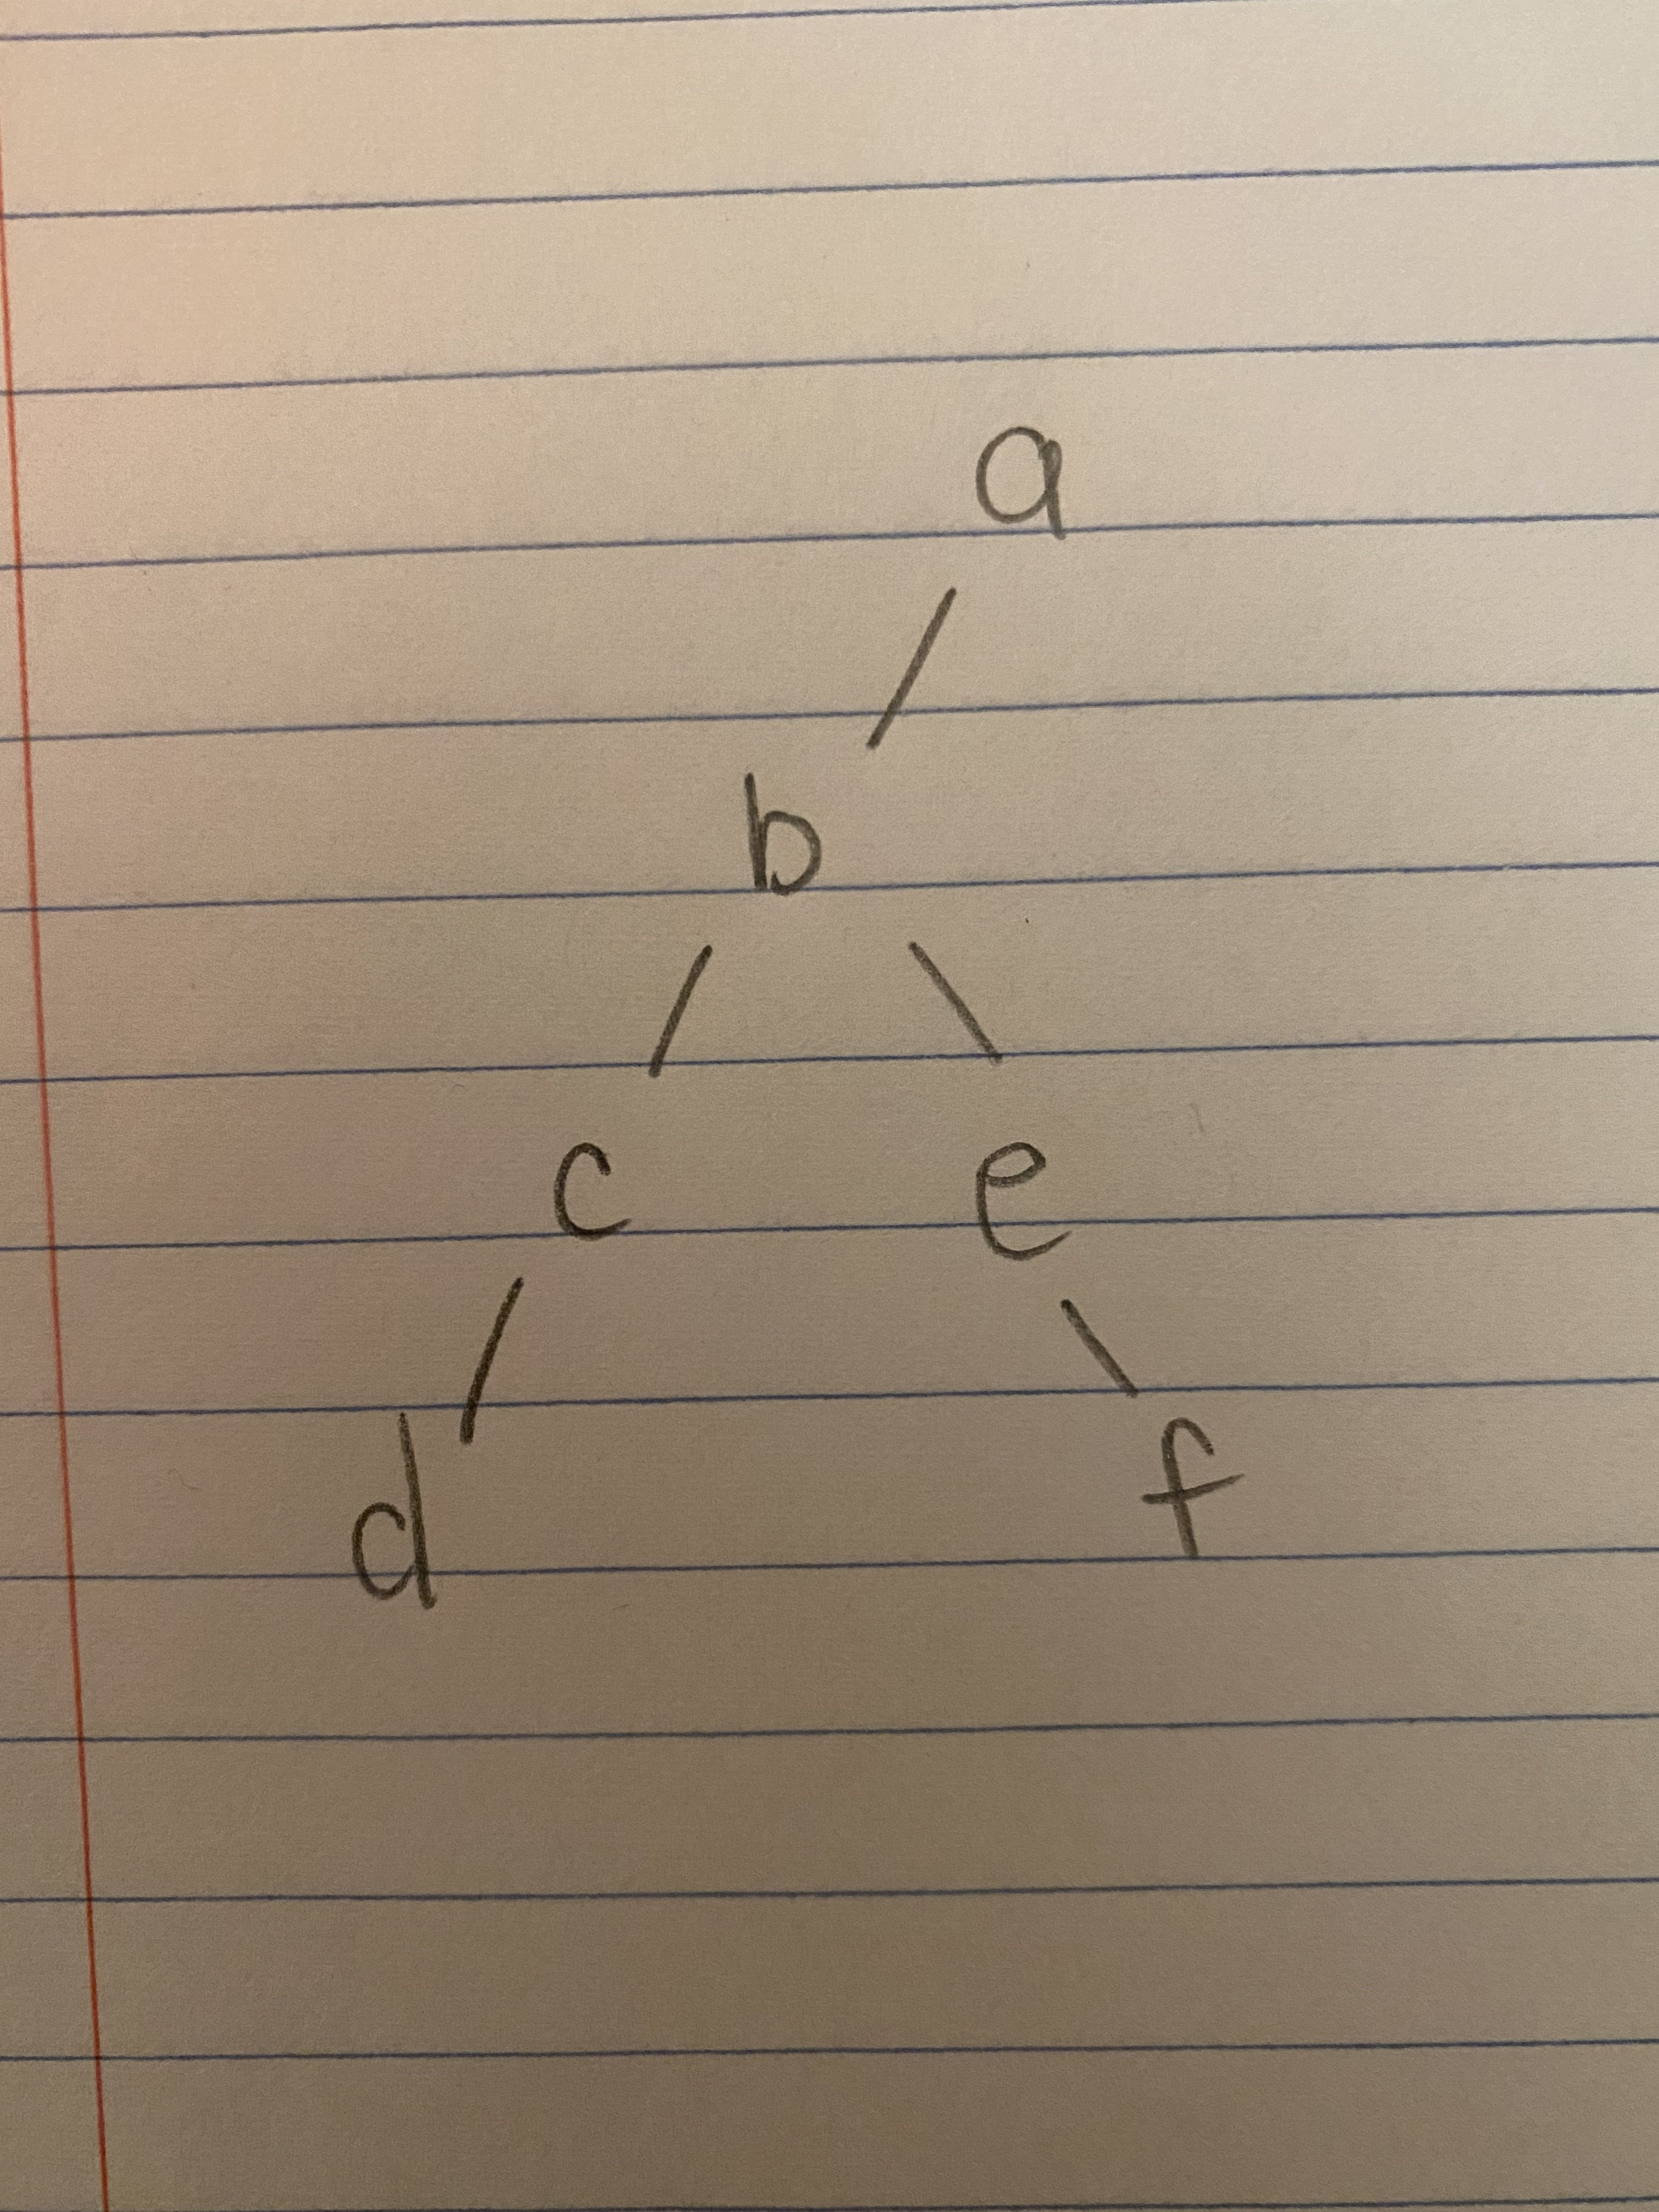
\includegraphics[scale=0.05]{csi2510lab3q2c3.png}\\
        
        
        
        
    \end{enumerate}
    
    
\end{enumerate}





\end{document} 
